%!TEX root=ast2016.tex

\begin{figure}[t]
  \centering

  \begin{tabular}{c c}

    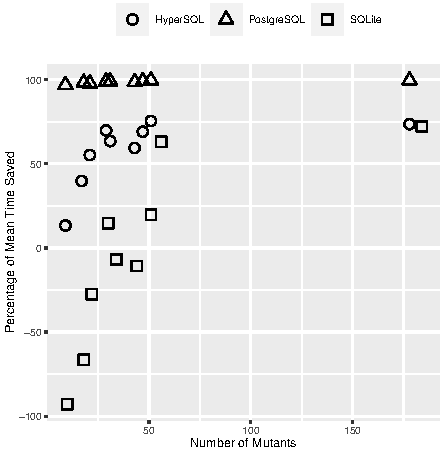
\includegraphics[scale=1.0]{graphics/graphic_scatterplot_nummutants_percentage.pdf} &

    % NOTE: This graph was removed to save space; it is slightly redundant and can be described in the text.
    % The caption now explains that the trend is the same for this graph; will also mention in the text.
    % 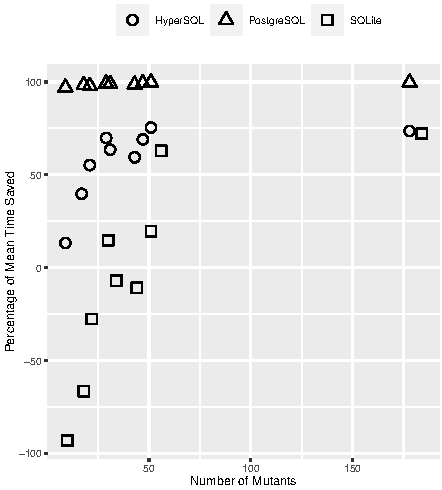
\includegraphics[scale=1.0]{graphics/graphic_scatterplot_numtests_percentage.pdf}

  \end{tabular}

  \caption{Scatter plot of the percentage of mean time saved for the number of schema mutants subject to analysis.}
  \label{fig:graphic_scatterplot_mutantstests_percentagetimesaved}

  {\small \justifying{ \noindent In these plots, a specific point corresponds to the percentage of mean time saved for a
  given number of mutants, across all three of the database management systems (a similar graph with the number of tests
  on the horizontal axis shows the same trend as this graph). For a detailed description of how to calculate the values on the
  vertical axis, please refer to Section~\ref{sec:experimental-setup}.  } \par}

  \vspace*{-1.25em}

\end{figure}
